


\section{Preliminary and Motivation}
\label{sec:analysis}

\subsection{Standard VLA Formulation and Its Limitation}


We consider a robot manipulation task where a policy $\pi$ maps multimodal observations and language instructions to actions. Let $\mathcal{O}$ be the observation space and $\mathcal{I}$ be the space of natural language instructions. A standard VLA policy $\pi_\theta\left(a_t \mid o_t, l\right)$ processes the current observation $o_t \in \mathcal{O}$ and instruction $l \in \mathcal{I}$ to predict an action $a_t \in \mathcal{A}$. The control task is thus formulated as:
% \vspace{-0.3em}
\begin{equation}
% a_t \sim \pi_\theta(a_t \mid o_t, l)
\pi_\theta\left(a_t \mid o_t, l\right).
\end{equation}
% \vspace{-0.1em}
where the model parameters $\theta$ are optimized on a large-scale dataset $\mathcal{D}$ collected under a set of specific system setups. In practice, $a_t$ is often structured as an action chunk to ensure temporal smoothness and control stability during execution.


This formulation embeds an implicit assumption: the system configuration 
$\psi$—encompassing camera viewpoints, mounting offsets, and the robot's 
morphological properties—is fixed and known. An ideal policy should instead 
condition on $\psi$ explicitly:
% \vspace{-0.3em}
\begin{equation}
\pi_\theta^*\left(a_t \mid o_t, l, \psi\right).
\end{equation}
Without $\psi$, training forces the model to marginalize over all 
configurations in the dataset:
% \vspace{-0.3em}
\begin{equation}
\pi_\theta\left(a_t \mid o_t, l\right) \approx \int \pi_\theta^*\left(a_t \mid o_t, l, \psi\right) 
p\left(\psi\right) d\psi.
\end{equation}
At deployment, when a specific $\psi'$ is realized, this averaged policy 
lacks the context to correctly interpret the observation-action correspondence, 
leading to degraded performance on novel configurations. This motivates 
explicit recovery of $\psi$ at test time.


\subsection{Interaction Context Enriches Configuration Information}
\label{subsec:theory}


We model robot-environment interaction as a POMDP where the latent state 
decomposes as $s_k = (\psi, \xi_k)$, with $\psi$ being the time-invariant 
system configuration and $\xi_k$ the time-varying scene state. The system 
evolves as:
\begin{equation}
s_0 \xrightarrow{a_1} s_1 \xrightarrow{a_2} \cdots \xrightarrow{a_t} s_t, 
\qquad o_k \sim p\left(o \mid s_k\right).
\end{equation}
We define the interaction context as $\mathcal{T} = \left(o_{0:t}, a_{1:t}\right)$ and 
analyze its information content under two mild assumptions: (A1) partial 
observability, $H\left(s_k \mid o_k\right) > 0$, a single image cannot uniquely identify 
the viewpoint or kinematics; and (A2) information-preserving transitions, 
$I\left(s_0; s_k \mid a_{1:k}\right) > 0$, state transitions preserve $\psi$, 
which holds since $\psi$ is time-invariant.

\textbf{Proposition 1.} \textit{Under A1 and A2, for any action sequence $a_{1:t}$, the interaction context 
$\mathcal{T}$ carries strictly more information about $\psi$ than any single 
observation:}
\begin{equation}
I\left(\psi;\, o_{0:t},\, a_{1:t}\right) > I\left(\psi;\, o_0\right).
\end{equation}



The proof is provided in \autoref{appendix:proof}. 
Since the result holds for any action distribution, 
task-agnostic random movements can also enrich the information 
available about $\psi$ despite carrying no task-specific information.



\begin{figure*}
    \centering
    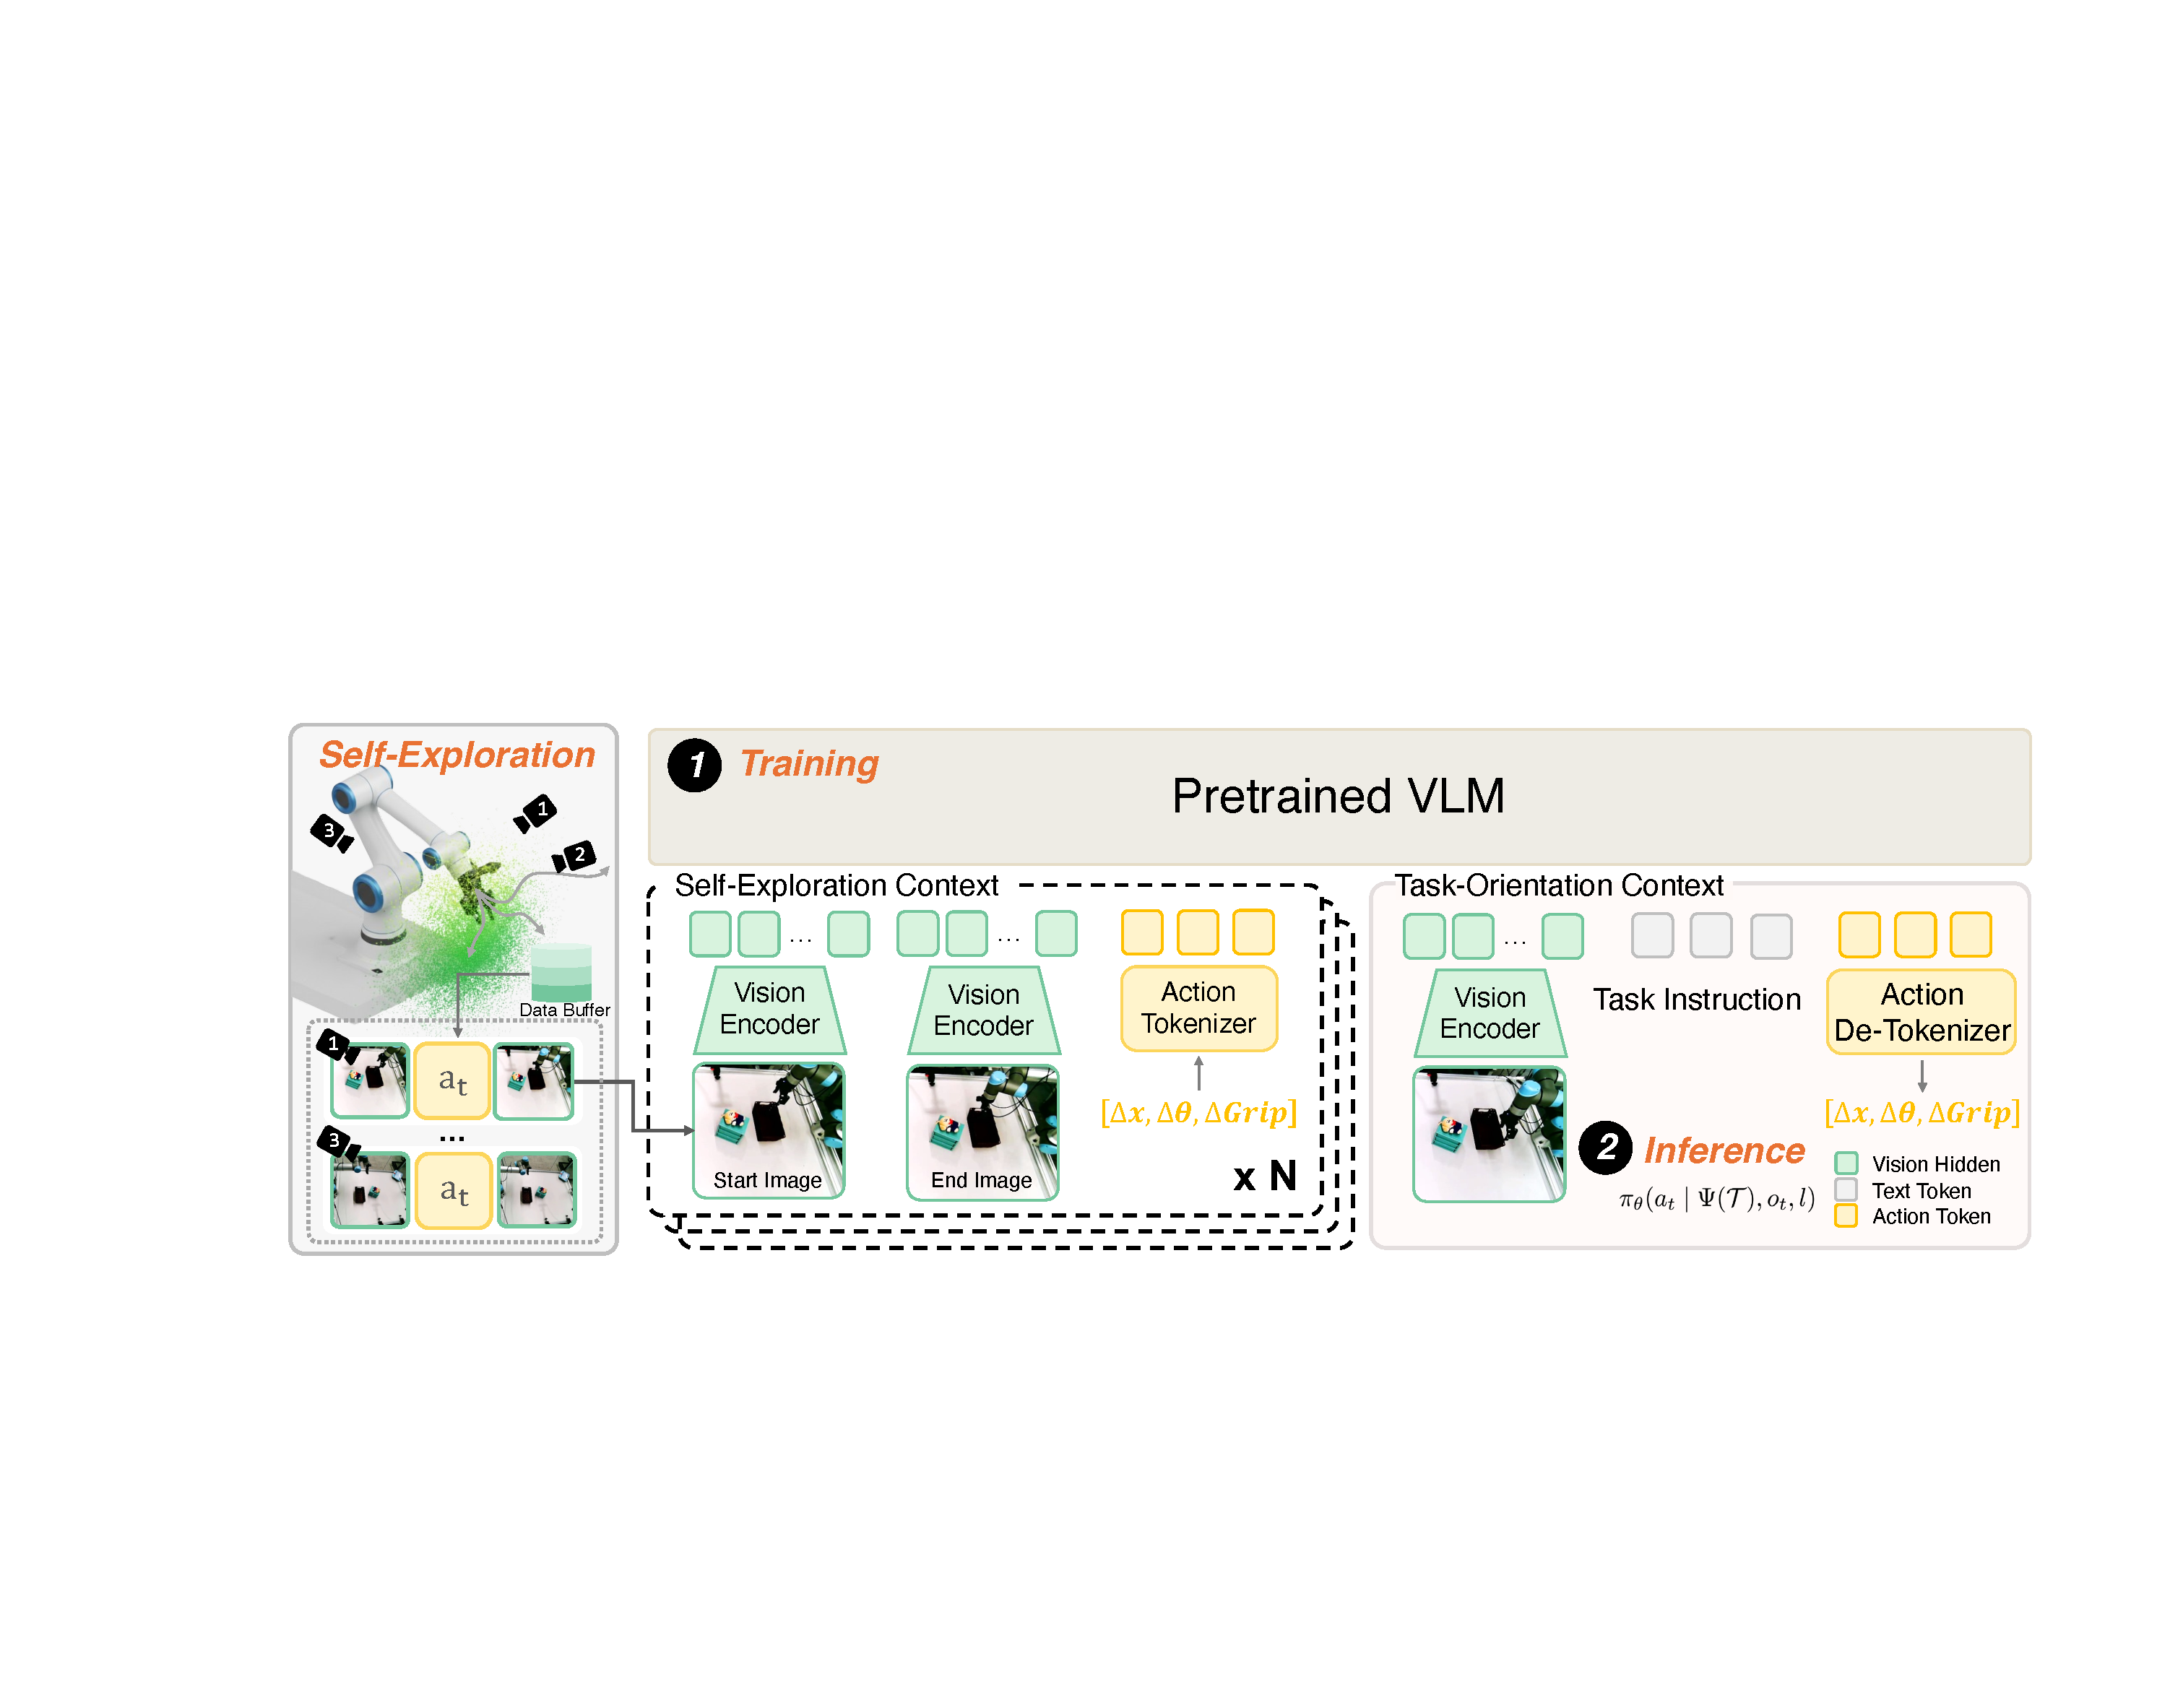
\includegraphics[width=1\linewidth]{imgs/method3-1.pdf}
    \caption{Overview of the ICWM Training and Inference Pipeline. (1) Training: The model is trained on data collected across diverse system configurations, where task-agnostic interaction clips are prepended to each training sample as context. (2) Inference: At test time, the robot first performs stochastic exploration to collect system context, which then guides the policy to generate precise actions via in-context inference.}
    \label{fig:methods}
    % \vspace{-4mm}
\end{figure*}





\section{In-Context World Modeling}
\label{sec:method}

To resolve the information incompleteness identified in \autoref{sec:analysis}, we introduce In-Context World Modeling (ICWM) (\autoref{fig:methods}). The core philosophy of ICWM is to transform the VLA from a static mapping into an adaptive inference mechanism that recovers the latent configuration $\psi$ through environmental interactions. 

Specifically, given a short history of task-agnostic interaction clips $\mathcal{T} = \left\{\left(o^s_i, a_i, o^e_i\right) \right\}_{i=1}^{N}$, the configuration can be inferred implicitly with a function $\Psi\left(\mathcal{T}\right)$. By conditioning the policy on interactions collected under the current configuration $\psi$, the policy is reformulated as:
\begin{equation}
a_t \sim \pi_\theta\left(a_t \mid \Psi \left(\mathcal{T}\right), o_t, l\right).
\end{equation}

The $\Psi\left(\mathcal{T}\right)$ term serves as a representation of the world dynamics under $\psi$, enabling the model to interpret $o_t$ in the context. This interaction-centric conditioning allows the policy to adapt its action selection to the specific visual and physical setup encountered at test time, thereby overcoming the generalization collapse of standard VLA models.


\subsection{In-Context Training}
\label{subsec:training}

To implement $\Psi\left(\mathcal{T}\right)$, we adopt a parameter-efficient design where $\Psi$ 
shares its parameters with the VLA backbone $\pi_\theta$, motivated by the structural symmetry between action prediction and configuration inference—both require understanding the correspondence between observations and actions. 

Each training sample is constructed by prepending $N$ task-agnostic interaction clips to the task query. 
These clips are randomly sampled from a pool of interaction segments collected across all training trajectories and viewpoints, ensuring diversity in the interaction context.
The model is trained on data collected across diverse system configurations, where the interaction context $\mathcal{T}$ naturally varies with the 
underlying $\psi$. This variation provides an implicit training signal: to accurately predict task actions across configurations, the model must learn to extract and utilize 
the dynamics information carried in $\mathcal{T}$, implicitly modeling the action-to-observation mapping under each specific system setup. The model is trained with 
the following loss:
\begin{equation}
\mathcal{L} = -\log \pi_\theta\left(a_t \mid \Psi\left(\mathcal{T}\right), o_t, l\right),
\end{equation}
where $\Psi\left(\mathcal{T}\right)$ denotes the hidden states induced by the 
interaction context. 


\subsection{Test-Time Active Probing and Inference}

At deployment, ICWM enables task-specific demonstration-free adaptation to novel system configurations through a two-phase inference protocol that requires no gradient updates, prior calibration, or knowledge of the target environment.

\textbf{Active Probing Phase.} 
Before task execution, the robot collects the interaction context $\mathcal{T} = \{\left(o^s_i, a_i, o^e_i\right)\}_{i=1}^N$ by performing $N$ task-agnostic probing actions. For each step $i \in \{1, \dots, N\}$, a random target pose is sampled within the robot's safe workspace, and the robot executes an action $a_i$ to reach it. The resulting transition $\left(o^s_i, a_i, o^e_i\right)$ is recorded. These probing movements are designed to be spatially diverse, sampling multiple directions relative to the end-effector's pose to provide sufficient coverage of the local dynamics manifold.
The probing workspace is defined to avoid contact with task-relevant objects, ensuring that the task initial state remains undisturbed throughout this phase.



\textbf{In-Context Execution Phase.} Once $\mathcal{T}$ is collected, the 
configuration inference function $\Psi$ processes the interaction context to implicitly recover the 
latent system configuration. Conditioned on the inferred hidden representation $\Psi\left(\mathcal{T}\right)$, the current observation $o_t$, and the language instruction $l$, the policy generates the task action $a_t \sim \pi_\theta\left(a_t \mid o_t, l, \Psi\left(\mathcal{T}\right)\right)$.
Since $\Psi$ shares parameters with the VLA backbone, this is implemented as a single forward pass where the Transformer first attends to $\mathcal{T}$, building configuration-aware hidden states, before processing the task query $\left(o_t, l\right)$ to produce actions aligned with the deployed physical setup.



